
\documentclass{article}


\usepackage{amsmath}
\usepackage{tikz}
\usepackage{float}
\usepackage{graphicx}
\usepackage{hyperref}

\usetikzlibrary{arrows}
\usetikzlibrary{positioning}

\begin{document}


\section{Experimental results and analysis}


\subsection{Experiments}

\subsubsection{Implementations}

We implement the algorithm on 3 POMDP problems: tiger, rock sample problem, 
and minesweeper game, which are discribed briefly as bellows:

\paragraph{Tiger problem:} There is 2 doors (left door and right door) for 
the agent to escape from the
room. However, there is only one door leading to the exit. There is a tiger 
behind the other door. The agent purpose is to open the door to exit, and 
to avoid the door containing the tiger. The agent can open the left door, 
open the right door, or to hear to the sound coming from the 2 doors. By 
hearing the sound, the agent can identify if the tiger is on the left door, 
or on the right door with the accuracy of 0.85. The cost for hearing action
is -1. The penalty for opening the door having the tiger is -100. The
reward for open the door to exit is +10.

The problem is modeled as 2 MDPs in Figure 1 and Figure 2.

\begin{figure}[h!] 
\centering

	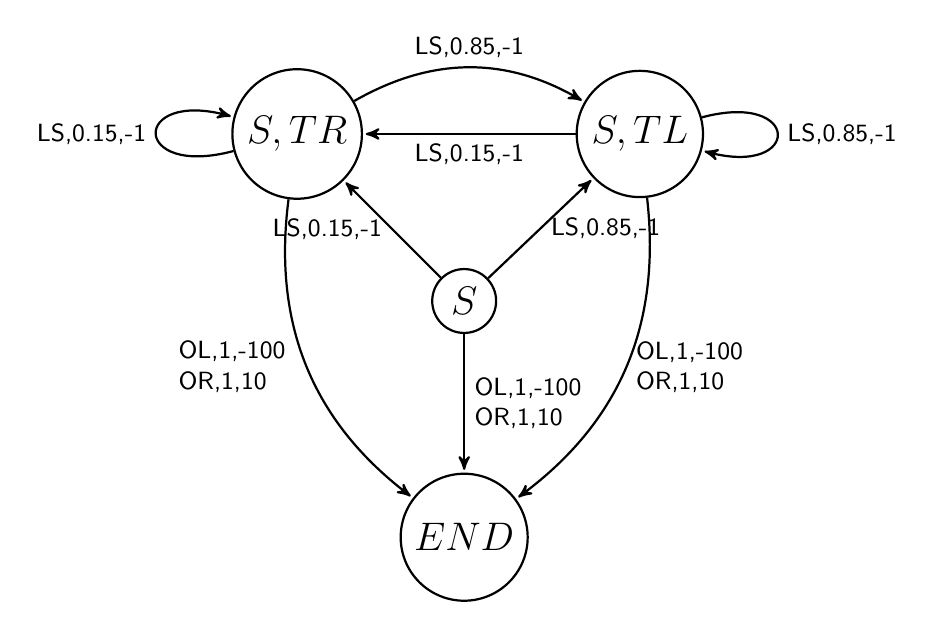
\begin{tikzpicture}[->,>=stealth',shorten >=1pt,auto,node distance=3cm,
	thick,main node/.style={circle,fill=white!20,draw,font=\sffamily\Large\bfseries}]

	\node[main node] (2) {$S,TR$};
	\node[main node] (1) [below right of=2] {$S$};
	\node[main node] (3) [right=2.7cm of 2] {$S,TL$};
	\node[main node] (4) [below of = 1] {$END$};

	\path[every node/.style={font=\sffamily\small}]
		(1) edge node [left] {LS,0.15,-1} (2)
			edge node [right] {LS,0.85,-1} (3)
			edge node [text width=1.5cm, align=left] {OL,1,-100\\OR,1,10} (4)
		(2) edge [loop left] node {LS,0.15,-1} (2)
			edge [bend left] node {LS,0.85,-1} (3)
			edge [bend right] node [text width=1.5cm, left] {OL,1,-100\\OR,1,10} (4)
		(3) edge [loop right] node {LS,0.85,-1} (3)
			edge node {LS,0.15,-1} (2)
			edge [bend left] node [text width=1.5cm, right] {OL,1,-100\\OR,1,10} (4);

	\end{tikzpicture}
	\caption{MDP Model for tiger on the left door}
	\label{fig:TigerLeftMdl}
\end{figure}

\begin{figure}[h!] 
\centering

	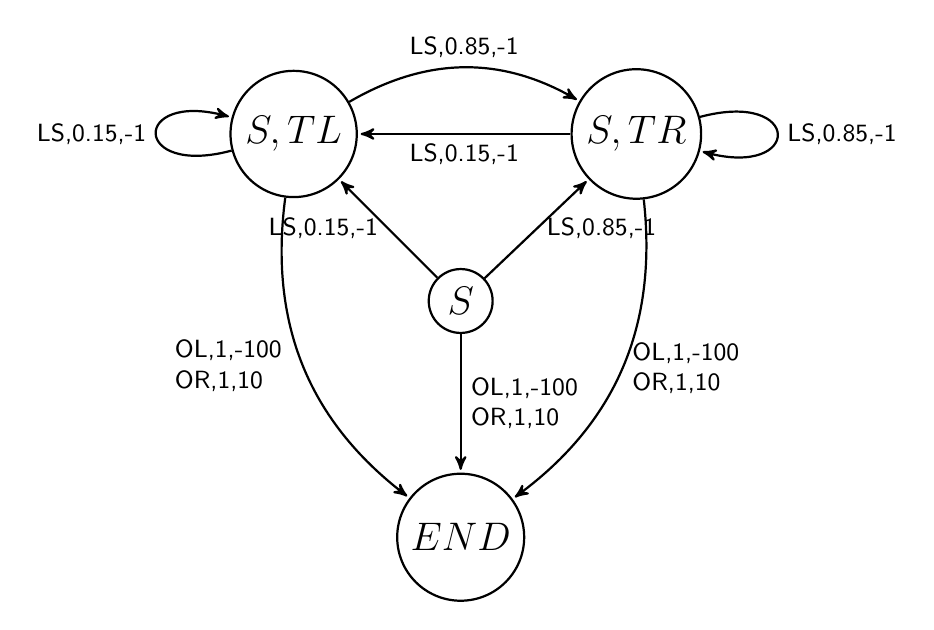
\begin{tikzpicture}[->,>=stealth',shorten >=1pt,auto,node distance=3cm,
	thick,main node/.style={circle,fill=white!20,draw,font=\sffamily\Large\bfseries}]

	\node[main node] (2) {$S,TL$};
	\node[main node] (1) [below right of=2] {$S$};
	\node[main node] (3) [right=2.7cm of 2] {$S,TR$};
	\node[main node] (4) [below of = 1] {$END$};

	\path[every node/.style={font=\sffamily\small}]
		(1) edge node [left] {LS,0.15,-1} (2)
			edge node [right] {LS,0.85,-1} (3)
			edge node [text width=1.5cm, align=left] {OL,1,-100\\OR,1,10} (4)
		(2) edge [loop left] node {LS,0.15,-1} (2)
			edge [bend left] node {LS,0.85,-1} (3)
			edge [bend right] node [text width=1.5cm, left] {OL,1,-100\\OR,1,10} (4)
		(3) edge [loop right] node {LS,0.85,-1} (3)
			edge node {LS,0.15,-1} (2)
			edge [bend left] node [text width=1.5cm, right] {OL,1,-100\\OR,1,10} (4);

	\end{tikzpicture}
	\caption{MDP Model for tiger on the right door}
	\label{fig:TigerRightMdl}
\end{figure}


\paragraph{Rock sample problem:} There is an environment represented by a 
grid of $m\times n$ cells, and an exit area on the right side of the grid. 
In this environment, there are $k$ rocks of type either good or bad. 
There is a rover at the starting position. The rover's task is to sample 
good rock and to move to the exit area. The position of $k$ rocks are known
to the rover, but the types of rocks is unknown. The rover is equipped with
a sensor to detect the type of rock with the accuracy of 
$0.5 + 0.5 \times 2^{-d/d_0}$, where $d$ is the distance from the rover to 
the checked rock, and $d_0$ is a constant. The rover can only sample a rock
at its position. If the rock is good, the rover receives reward of 10. If the 
rock is bad, the rover receives reward of -10. Apart from checking, and sampling, 
the rover can move north, east, west, south in the grid. There is high cost for 
moving out of the grid. Moving to exit areas yields reward of 10.

In our experiment, there are 7 rows and 8 columns. There are 8 rocks
locating at $\{(0,1), (1,1), (1,4), (1,6), (3,6), (4,3), (6,1), (6,5)\}$
(Figure 3).

\begin{figure}[h!]
\centering
\includegraphics[width=0.5\textwidth]{rocksample.png}
\caption{Rock Sample problem}
\label{fig:RockSampleProb}
\end{figure}

In this problem, the probability of a rock is good (or bad) is independent from one
rock to another. Hence, instead of having a state as a tuple 
$(S_{x,y},R_{0,status}, R_{1,status}, \dots, R_{7,status})$, 
where $S_{x,y} \in \{s_{0,0}, s_{0,1}, \dots, s_{7,7}\}$ 
is the position of the rover, $R_{i,status} \in \{r_{i,bad}, r_{i,good}\}$,
$i=0,1,\dots,7$ are the rocks' status; we model each status as a tuple
$(S_{x,y},R_{i,status})$ (since each action of the rover can only
affect one rock status distribution at a one time). This reduces the computation
of the program. Hence, we directly model the mean MDP as bellows:

\begin{itemize}

\item Belief: $b(i), i=0,1,2,\dots,7$ is the probability of the 
i\textsuperscript{th} rock's status being good

\item States: $\{(S_{x,y},R_{i,status}), S_{x,y}\}$ (states with observation, and 
states without observation)

\item Actions: $\{north, east, west, south, sampling, check_i\}, i=0,1,2,\dots,7$ 
($check_i$ means checking the i\textsuperscript{th} rock's status)

\item Transition functions:
	\begin{itemize}
	\item Moving action (north, east, west, south) is deterministic and only changes
	the rover's position.\\ 
	E.g., $P( (S_{x+1,y},R_{0,good}) | (S_{x,y},R_{0,good}, south) ) = 1.0$,\\
	$P( S_{x+1,y} | S{x,y}, south) = 1.0$
	\item Samping action: $P( S_{x,y} | (S_{x,y}, R_{i,status}), sample) = 1.0$,\\
	$P( S_{x,y} | S_{x,y}, sample) = 1.0$
	\item Checking action:\\
	$P( (S_{x,y}, R_{i,good}) | (S_{x,y}, R_{j,status}, check_i) ) = \alpha = b(i)acc(S_{x,y}, i) + (1 - b(i))(1 - acc(S_{x,y}))$, where $acc(S_{x,y},i)$ is the accuracy 
	of sensor given the rover at $(x,y)$ and checking the \textsuperscript{th} rock.\\
	$P( (S_{x,y}, R_{i,bad}) | (S_{x,y}, R_{j,status}, check_i) ) = 1 - \alpha$
	\end{itemize}

\item Reward functions: Only action sampling and moving resulting in rewards as bellows.
	\begin{itemize}
	\item Moving action (deterministic): If the rover goes to exit area, it receives a 
	reward of 10. If the rover goes out of the grid (not exit area), it receives a
	penalty of -1000.
	\item Sampling action: $R(S_{x,y}, sample) = 10 \times b(i) - 10 \times (1 - b(i))$,
	where $i$ is the index of the sampled rock.
	\end{itemize}

\end{itemize}


\paragraph{Minesweeper game:} There is a grid of cells. Each cell can contain at most 1 mine.
There are $k$ mines whose locations are unknown to the player in the grid. The player could choose to 
reveal a cell. If the cell revealed contains a mine, the player loses the game. If the cell 
revealed does not contain a mine, there are 2 cases: (1) if there are $x$ mines in 8 cells 
surrounding the revealed cell, the revealed cell shows $x$; (2) if there are no mines in 8 
cells surrounding the revealed cell, the surrounding cells are revealed with the same rule 
applied to player-reveal cells. The player could choose to mark a cell if he/she thinks it
contains a mine. The player wins the game if all mine-free cells are revealed.


\subsubsection{Results}

\begin{table}[H]
\caption{Rock Sample results}
\begin{center}
	\begin{tabular} {| l | c | c |}
		\hline
			& Execution time (ms) & Total reward\\ 
		\hline
		SARSOP & 400,000 & 21.27\\
		HSVI-BFS (using BPVI as lower bound) & 826 & 21.46\\
		HSVI-BFS (using blind policy as lower bound) & 954 & 17.10\\
		AEMSI (using BPVI as lower bound) & 954 & 17.10\\
		AEMSI (using blind policy as lower bound) & 900 & 10.30\\
		Our algorithm & 300 & 18.15\\ 
		\hline
	\end{tabular}
\end{center}
\end{table}


\subsection{Analysis}

\emph{NEED MORE DETAILED AND CONCRETE ANALYSIS OF EXPERIMENTS.}


\section{Conclusions and future work}

\paragraph{Advantages} Our algorithm gives better running time compared with
other POMDP algorithms.
\paragraph{Disadvantages} There are two main disadvantages of our algorithm: (1)
it can only be applied to a limited domain of POMDP problem of discrete and 
static unobservable states; (2) to obtain good policy, our algorithm requires
to tune the value of reward bonus discount.
\paragraph{Future work:} We can investigate how to handle the dynamic environment, and how to choose reward bonus discount so that we get better policy.


\begin{thebibliography}{9}

\bibitem{smith}
	T Smith, R Simmons. \emph{Heuristic search value iteration for POMDPs} - Proceedings of the 20\textsuperscript{th} conference on Uncertainty in AI, 2004.

\bibitem{kurn}
	H Kurniawati, D Hsu, WS Lee. \emph{SARSOP: Efficient Point-Based POMDP Planning by Approximating Optimally Reachable Belief Spaces} - Robotics: Science and Systems, 2008.

\bibitem{kolter}
	Z Kolter and A Y Ng. \emph{Near-bayesian exploration in polynomial time} - In Proceedings to International Conference on Machine Learning, 2009.

\bibitem{sorg}
	Sorg, S Singh, and RL Lewis. \emph{Variance-based rewards for approximate Bayesian reinforcement learning} - In Proceedings to Uncertainty in AI, 2010.

\end{thebibliography}

\end{document}
